\chapter{METODOLOGIA}

Nesta seção está expressa a abordagem metodológica utilizada na elaboração da rotina em Python contendo uma interface gráfica, em conjunto com o cálculo dos indicadores determinados pelo Módulo 8 do PRODIST. Segue uma divisão em etapas lógicas, que contemplam desde o planejamento e estruturação até a validação dos resultados obtidos.

\section{DESENVOLVIMENTO DA ROTINA EM PYTHON}

\subsection{Escolha da linguagem de programação}

A linguagem Python foi escolhida por ser de fácil manuseio e possuir grandes variedades de bibliotecas voltadas a análise de dados e construção de interfaces.

\subsection{Arquitetura}

Para implementação da rotina foi escolhido utilizar uma abordagem modular e composta por classes, facilitando a organização e manutenção do código. A arquitetura geral pode ser dividida em 3 partes principais: a interface gráfica, as classes para cálculo dos indicadores e uma classe geral de controle das análises dos indicadores.

\subsection{Implementação das classes}

Foram desenvolvidas classes para cada tipo de indicador determinado pelo Módulo 8 PRODIST, onde cada uma fica responsável por realizar os cálculos específicos para seu indicador. As classes foram desenvolvidas para os indicadores:

\begin{itemize}
  \item variação de tensão (DRC e DRP);
  \item fator de potência: verificar se os valores de fator de potência estão condizentes com os níveis adequados;
  \item distorções harmônicas ($DTT95\%$, $DTT_p95\%$, $DTT_i95\%$ e $DTT_395\%$);
  \item desequilíbrio de tensão ($FD95\%$);
  \item variação de frequência: verificar se os valores das frequências estão dentro da faixa adequada.
\end{itemize}

A classe geral de controle das análises age como um intermediário entre a interface gráfica e as classes que calculam os indicadores, capitando os parâmetros de entrada fornecidos pela interface e selecionado qual classe de indicador será instanciada.

\subsection{Uso de bibliotecas específicas}

Dentre as bibliotecas mais utilizadas nesse trabalho se destacam:

\begin{itemize}
  \item Pandas: utilizada para análise dos dados, XLS ou CSV, colhidos pelo analisador de QEE;
  \item NumPy: utilizada para verificação das informações contidas dentro dos arquivos, calculando valores de percentis ou tamanho das bases de dados;
  \item Matplotlib: utilizado para geração de gráficos das tensões;
  \item PySide6: utilizada para a criação da interface gráfica responsável pela visualização e manuseio da rotina elabora na linguagem Python.
\end{itemize}

\section{INTERFACE GRÁFICA}

\subsection{Desenvolvimento}

Foi desenvolvido uma estrutura modular para geração da interface gráfica através da biblioteca PySide6, por ser uma biblioteca de código aberto e de alta personalização.

\subsection{Funcionalidades}

A interface gráfica permite que o usuário interaja com a rotina criada, importando uma planilha CSV ou XLS, para uma tabela e selecione os parâmetros que deseja para calcular os indicadores.

A interface consegue visualizar gráficos das tensões medidas e gerar um relatório em pdf com os valores dos indicadores calculados, além de salvar os valores dos indicadores em formatos diferentes, seja TXT, JSON, CSV ou XLS.

\subsection{Layout prévio}

O layout prévio da interface segue a \autoref{fig:main_windown}, em que possui uma tabela, para mostrar os dados importados da planilha, e uma barra na lateral direita, onde conterá os resultados da análise dos indicadores.

\begin{figure}[H]
	\centering
	\caption{\textit{Layout} da interface gráfica}
	\label{fig:main_windown}
	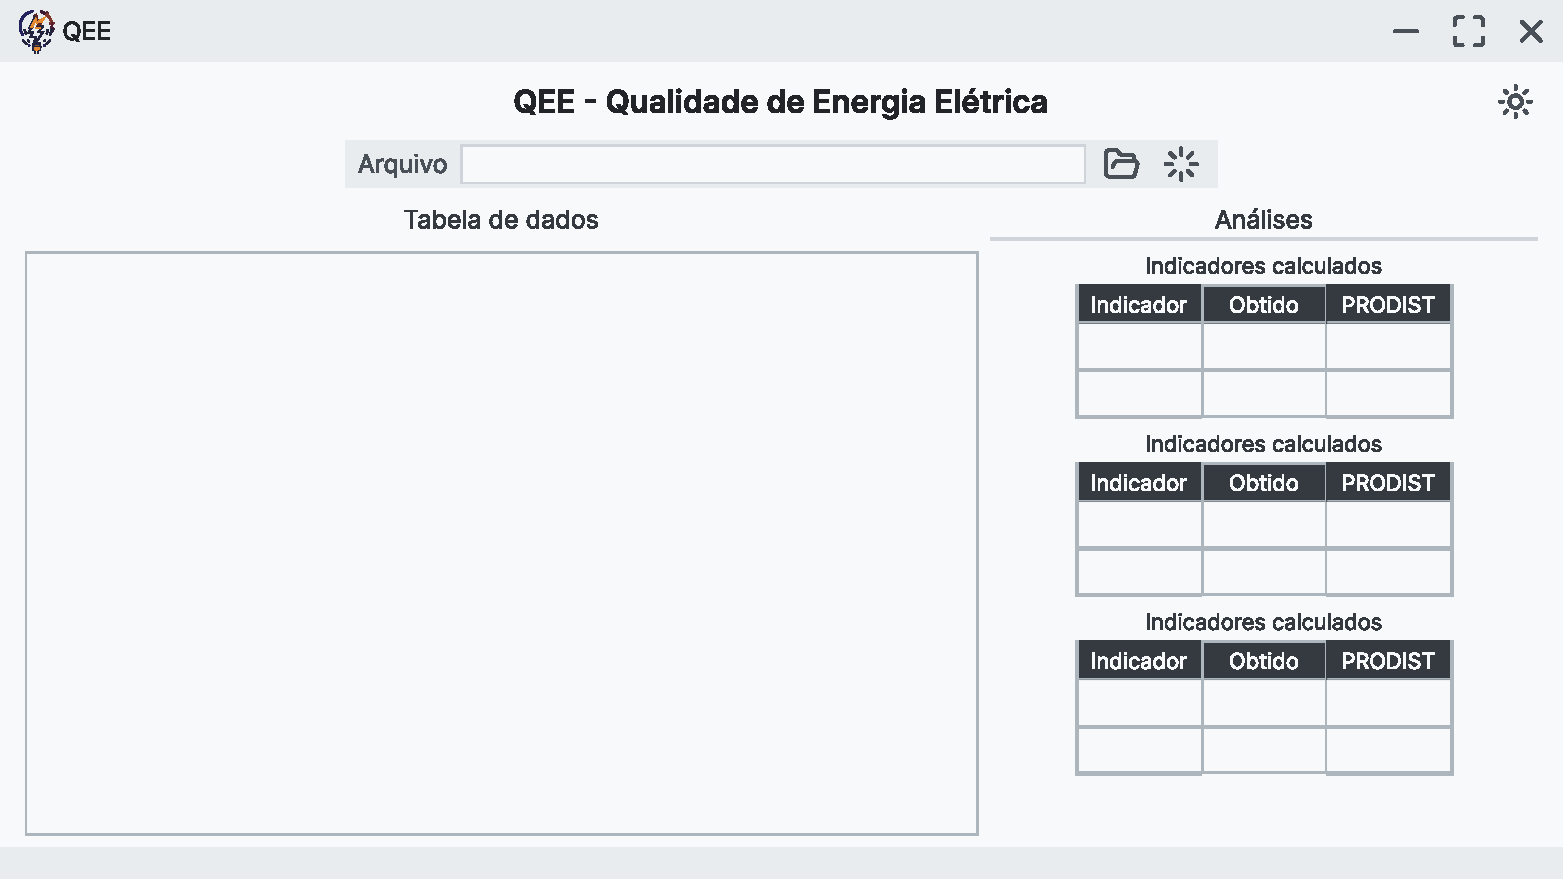
\includegraphics[width=16cm]{illustrations/figures/main_windown.pdf}
	\fonte{Autoria própria}
\end{figure}

\section{COLETA DE DADOS}

\subsection{Analisador de qualidade}

Existem vários modelos de analisadores de qualidade de energia, dentre eles o instrumento MINIPA modelo ET-5061C, é um analisador de rede construído pelo fabricante MINIPA respeitando a norma de segurança EN-61010. Esse dispositivo consegue visualizar em tempo real parâmetros elétricos, mostra sinais em forma de gráficos, histogramas, diagramas vetoriais e consegue salvar esses dados para que possam ser visualizados e analisados em outros softwares \cite{ref:minipa_2019}. Na \autoref{fig:analisador_qee} apresenta-se um exemplo desse modelo.

\begin{figure}[H]
	\centering
	\caption{Analisador de qualidade de energia elétrica MINIPA modelo ET-5061C}
	\label{fig:analisador_qee}
	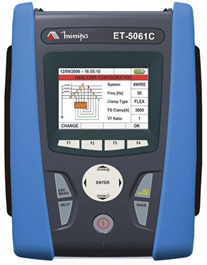
\includegraphics[width=5.5cm]{illustrations/figures/analisador_qee.png}
	\fonte{\citeonline{ref:minipa_2019}}
\end{figure}

\subsection{Fonte de dados}

Os dados colhidos para análise da ferramenta, foram obtidos por meio de um analisador de QEE instalado no bloco de professores I desta universidade. O estudo da fonte de dados teve o objetivo de compreender os aspectos organizacionais e gerar a rotina de importação e análise desses dados, buscando padrões que tornem essa rotina adequada a quaisquer medições realizadas.

\subsection{Processamento dos dados}

Antes da análise, os dados foram pré-processados e selecionados apenas as 1008 leituras válidas, conforme determinado pelo PRODIST. Também foram unidas todas as planilhas, extraídas do analisador de QEE, em uma única planilha (XLS ou CSV) com todos os valores medidos.

\section{ANÁLISE DE DADOS}

\subsection{Uso das classes implementadas}

Com a planilha única criada, os valores foram importados para a classe geral de controle das análises, através da interface gráfica, e convertida em um DataFrame para ser usado dentro das funções que instanciam as classes para cálculo dos indicadores. Nessas funções, além da instância das classes de indicadores, os valores dos DataFrame são convertidos em listas de valores numéricos para que as classes pré-determinadas possam executar os cálculos dos indicadores.

\subsection{Interpretação dos resultados}

Consistiu na comparação dos indicadores calculados com os fornecidos pelo PRODIST. Permitindo assim determinar a situação da qualidade de energia da unidade consumidora analisada.
